Dans un triangle $ABC$, on note $a = BC$, $b = CA$, $c = AB$. Les
bissectrices intérieures $(AD)$, $(BE)$ et $(CF)$, avec $D \in [BC]$,
$E \in [CA]$ et $F \in [AB]$, sont concourantes en $I$, centre du cercle
inscrit. On veut démontrer que
\[
\frac14 < \frac{AI}{AD} \cdot \frac{BI}{BE} \cdot \frac{CI}{CF} \leqslant \frac{8}{27}
\qquad \text{(OIM 1991)}.
\]

\begin{center}
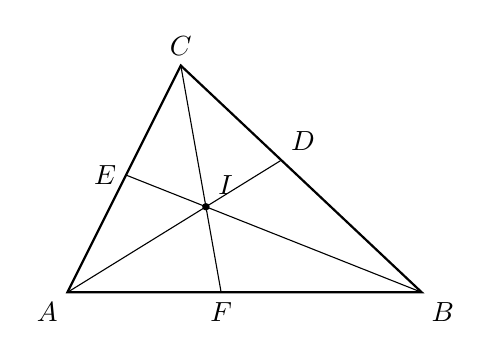
\begin{tikzpicture}[scale=0.9]
  \coordinate (A) at (0,0);
  \coordinate (B) at (5,0);
  \coordinate (C) at (1.6,3.2);
  % Pieds des bissectrices (théorème de la bissectrice) et centre inscrit,
  % calculés pour A(0;0), B(5;0), C(1,6;3,2).
  \coordinate (D) at (3.018,1.865);
  \coordinate (E) at (0.827,1.655);
  \coordinate (F) at (2.169,0);
  \coordinate (I) at (1.954,1.208);
  \draw[thick] (A) -- (B) -- (C) -- cycle;
  \draw (A) -- (D) (B) -- (E) (C) -- (F);
  \fill (I) circle (1.5pt);
  \node[below left] at (A) {$A$};
  \node[below right] at (B) {$B$};
  \node[above] at (C) {$C$};
  \node[above right] at (D) {$D$};
  \node[left] at (E) {$E$};
  \node[below] at (F) {$F$};
  \node[above right=1pt] at (I) {$I$};
\end{tikzpicture}
\end{center}

\begin{enumerate}
  \item À l'aide du théorème de la bissectrice ($BD/DC = c/b$), montrer que
  \[
  BD = \frac{ac}{b+c} \qquad\text{et}\qquad CD = \frac{ab}{b+c}.
  \]
  \item Dans le triangle $ACD$, la droite $(CI)$ est la bissectrice de
  l'angle $\widehat{ACD}$. En déduire que $\dfrac{AI}{ID} = \dfrac{b+c}{a}$,
  puis que
  \[
  \frac{AI}{AD} = \frac{b+c}{a+b+c}.
  \]
  Écrire, sans nouveau calcul, les formules analogues pour $BI/BE$ et $CI/CF$.
  \item On pose $P = \dfrac{AI}{AD} \cdot \dfrac{BI}{BE} \cdot \dfrac{CI}{CF}$.
  Exprimer $P$ en fonction de $a$, $b$, $c$, puis appliquer l'inégalité
  arithmético-géométrique aux trois nombres $b+c$, $c+a$, $a+b$ pour obtenir
  $P \leqslant 8/27$. Quand y a-t-il égalité ?
  \item \emph{Minoration.} On utilise la forme IV de l'inégalité
  triangulaire : $a = y+z$, $b = z+x$, $c = x+y$ avec $x, y, z > 0$. On pose
  \[
  r = \frac{x}{x+y+z}, \qquad s = \frac{y}{x+y+z}, \qquad t = \frac{z}{x+y+z}.
  \]
  Montrer que $\dfrac{AI}{AD} = \dfrac{1+r}{2}$, puis développer
  $(1+r)(1+s)(1+t)$ en utilisant $r+s+t = 1$ et conclure que $P > 1/4$.
  \item \emph{Pour aller plus loin.} Montrer que la borne $1/4$ ne peut pas
  être remplacée par un nombre plus grand.
\end{enumerate}
